% Options for packages loaded elsewhere
\PassOptionsToPackage{unicode}{hyperref}
\PassOptionsToPackage{hyphens}{url}
%
\documentclass[
]{book}
\usepackage{amsmath,amssymb}
\usepackage{iftex}
\ifPDFTeX
  \usepackage[T1]{fontenc}
  \usepackage[utf8]{inputenc}
  \usepackage{textcomp} % provide euro and other symbols
\else % if luatex or xetex
  \usepackage{unicode-math} % this also loads fontspec
  \defaultfontfeatures{Scale=MatchLowercase}
  \defaultfontfeatures[\rmfamily]{Ligatures=TeX,Scale=1}
\fi
\usepackage{lmodern}
\ifPDFTeX\else
  % xetex/luatex font selection
\fi
% Use upquote if available, for straight quotes in verbatim environments
\IfFileExists{upquote.sty}{\usepackage{upquote}}{}
\IfFileExists{microtype.sty}{% use microtype if available
  \usepackage[]{microtype}
  \UseMicrotypeSet[protrusion]{basicmath} % disable protrusion for tt fonts
}{}
\makeatletter
\@ifundefined{KOMAClassName}{% if non-KOMA class
  \IfFileExists{parskip.sty}{%
    \usepackage{parskip}
  }{% else
    \setlength{\parindent}{0pt}
    \setlength{\parskip}{6pt plus 2pt minus 1pt}}
}{% if KOMA class
  \KOMAoptions{parskip=half}}
\makeatother
\usepackage{xcolor}
\usepackage{longtable,booktabs,array}
\usepackage{calc} % for calculating minipage widths
% Correct order of tables after \paragraph or \subparagraph
\usepackage{etoolbox}
\makeatletter
\patchcmd\longtable{\par}{\if@noskipsec\mbox{}\fi\par}{}{}
\makeatother
% Allow footnotes in longtable head/foot
\IfFileExists{footnotehyper.sty}{\usepackage{footnotehyper}}{\usepackage{footnote}}
\makesavenoteenv{longtable}
\usepackage{graphicx}
\makeatletter
\def\maxwidth{\ifdim\Gin@nat@width>\linewidth\linewidth\else\Gin@nat@width\fi}
\def\maxheight{\ifdim\Gin@nat@height>\textheight\textheight\else\Gin@nat@height\fi}
\makeatother
% Scale images if necessary, so that they will not overflow the page
% margins by default, and it is still possible to overwrite the defaults
% using explicit options in \includegraphics[width, height, ...]{}
\setkeys{Gin}{width=\maxwidth,height=\maxheight,keepaspectratio}
% Set default figure placement to htbp
\makeatletter
\def\fps@figure{htbp}
\makeatother
\setlength{\emergencystretch}{3em} % prevent overfull lines
\providecommand{\tightlist}{%
  \setlength{\itemsep}{0pt}\setlength{\parskip}{0pt}}
\setcounter{secnumdepth}{5}
\usepackage{booktabs}
\usepackage{amsthm}
\makeatletter
\def\thm@space@setup{%
  \thm@preskip=8pt plus 2pt minus 4pt
  \thm@postskip=\thm@preskip
}
\makeatother

\usepackage{tcolorbox}
\tcbuselibrary{breakable}

\newtcolorbox{blackbox}{
  colback=black,
  coltext=white,
  colframe=black,
  boxsep=5pt,
  arc=4pt,
  breakable
  }
\newtcolorbox{bonus}{
  colback=blue!15,
  colframe=blue!15,
  coltext=black!80,
  boxsep=5pt,
  arc=4pt,
  breakable
  }
\newtcolorbox{reflect}{
  colback=green!5,
  colframe=green!5,
  coltext=black!80,
  boxsep=5pt,
  arc=4pt,
  breakable
  }
\newtcolorbox{assessment}{
  colback=blue!5,
  colframe=blue!5,
  coltext=black!80,
  boxsep=5pt,
  arc=4pt,
  breakable
  }
  
\newtcolorbox{progress}{
  colback=purple!10,
  colframe=purple!10,
  coltext=black!80,
  boxsep=5pt,
  arc=4pt,
  breakable
  }
\newtcolorbox{video}{
  colback=yellow!5,
  colframe=yellow!5,
  coltext=black!80,
  boxsep=5pt,
  arc=4pt,
  breakable
  }
\newtcolorbox{caution}{
  colback=red!5,
  colframe=red!5,
  coltext=black!80,
  boxsep=5pt,
  arc=4pt,
  breakable
  }
\newtcolorbox{feedback}{
  colback=black!5,
  colframe=black!5,
  coltext=black!80,
  boxsep=5pt,
  arc=4pt,
  breakable
  }
\ifLuaTeX
  \usepackage{selnolig}  % disable illegal ligatures
\fi
\usepackage[]{natbib}
\bibliographystyle{apalike}
\IfFileExists{bookmark.sty}{\usepackage{bookmark}}{\usepackage{hyperref}}
\IfFileExists{xurl.sty}{\usepackage{xurl}}{} % add URL line breaks if available
\urlstyle{same}
\hypersetup{
  pdftitle={phil210-GX},
  pdfauthor={Name},
  hidelinks,
  pdfcreator={LaTeX via pandoc}}

\title{phil210-GX}
\author{Name}
\date{}

\begin{document}
\maketitle

{
\setcounter{tocdepth}{1}
\tableofcontents
}
\hypertarget{welcome}{%
\chapter*{Welcome}\label{welcome}}
\addcontentsline{toc}{chapter}{Welcome}

This is the course book for {[}insert{]}. This book is divided into 6 units of study to help you engage with the materials. The course resources and learning activities are designed not only to help prepare you for the course assessments, but also to give you opportinities to practice various skills.

Below you will find information about how to navigate this book. Please also refer the schedule in Moodle, as well as the Asseessment section in Moodle for instructions on required readings and assignments.

\hypertarget{course-notes}{%
\section*{Course Notes}\label{course-notes}}
\addcontentsline{toc}{section}{Course Notes}

You should be reading this information in the context of a Trinity Western University course offered via Moodle. If this is not the case, then this may be an unauthorized reproduction of the course. Please contact \href{mailto:elearning@twu.ca}{\nolinkurl{elearning@twu.ca}} if you have concerns.

These notes will be your guide through the learning activities and assessment strategies necessary for you to succeed in the course, so it is important for you to engage to the best of your ability and take advantage of the resources available to you through Trinity Western University.

Assessment tasks are managed in other sections of the Moodle course, so be sure to familiarize yourself with those requirements and resources.

\hypertarget{how-this-course-is-built}{%
\section*{How this Course is Built}\label{how-this-course-is-built}}
\addcontentsline{toc}{section}{How this Course is Built}

This course is primarily designed to be completed asynchronously, meaning that there are no scheduled times or places that you are required to meet, even online. You can work according to your own schedule \emph{within the six weeks you have to complete the course}. That said, this is a full university level course and there are timelines that we strongly recommend that you meet to ensure that you are succeeding in building your knowledge through the course.

It would be to your significant disadvantage to submit everything at the end of the course.

Asynchronous courses require learners to be well-organized and self-motivated, and we have included supports for you to help you develop strong learning habits that will ensure your success.

For example, there are several self-check quizzes throughout the course. These quizzes are not graded, but they can be powerful tools for you to ensure you understand key ideas and concepts. We suggest you take each quiz without the aid of your notes and textbook and multiple times until you have mastered the content. This strategy taps into three powerful learning structures that have been shown to be highly effective.

\begin{enumerate}
\def\labelenumi{\arabic{enumi}.}
\tightlist
\item
  \textbf{Effortful recall.} By intentionally trying to recall information without external aids, you are strengthening the neural pathways in your brain that lead to building new connections between ideas. One way to make recall easier is to connect key ideas to other things that you know or have experienced. For example, you might be studying World War II, and you connect the date that Canadians participated in the D-Day operation with something else meaningful to you that happened on June 6, like maybe the date you bought your first car.\\
\item
  \textbf{Spaced repetition.} By spreading out your attempts on the quiz (leaving a few days between attempts) you can maximize the effects of the first strategy (effortful recall) and ensure that your second or third attempts truly reflect what you know about the topic. We suggest leaving 1-3 days between attempt 1 and 2, then 4-5 days between attempt 2 and 3. You can use a tool like Trello, Notion, or Asana (free versions), or even a task list on your phone to set up a spaced repetition schedule.\\
\item
  \textbf{Interleaving.} This is the practice of studying a particular topic for a relatively short period of time (maybe 30-40 mins), then switching to a different topic for the same period, before going back to the original topic. We will help build this into your learning by including items from unit 1 in your unit 2-6 quizzes. You can also practice this by taking regular breaks in your work, or even by retaking a unit 1 quiz while you are working in unit 2.
\end{enumerate}

These three strategies are very effective at helping people \emph{remember} key facts about a particular topic, an important first step in learning at the university level. However, you will be asked to do much more than just remember facts. Your ultimate goal is to develop \textbf{evaluative judgement}, or the ability for you to judge for yourself the quality of your (or your peers') responses to prompts.

The discussion forums are a key way for you to do this. We have set up the forums in such a way that you will need to present a response to any given prompt before you see other learners' responses. We strongly encourage you to use this structure to formulate your own ideas before you present them in the forum, and then to use the responses of your peers to help you evaluate your own response.

Using these self-check activities in this way is designed to help you to succeed on the course assignments, upon which your final grade will be determined. These assignments will require you to \textbf{use} the facts of the course to generate unique responses to the prompts, based on your past experiences, knowledge, and ability to evaluate the quality of your own work.

\hypertarget{how-to-navigate-this-book}{%
\subsection*{How To Navigate This Book}\label{how-to-navigate-this-book}}
\addcontentsline{toc}{subsection}{How To Navigate This Book}

To move quickly to different portions of the book, click on the appropriate chapter or section in the table of contents on the left. The buttons at the top of the page allow you to show/hide the table of contents, search the book, change font settings, download a pdf or ebook copy of this book, or get hints on various sections of the book.


\includegraphics{assets/course-intro/menu.png}

The faint left and right arrows at the sides of each page (or bottom of the page if it's narrow enough) allow you to step to the next/previous section. Here's what they look like:


\includegraphics{assets/course-intro/left_arrow.png} 
\includegraphics{assets/course-intro/right_arrow.png}

You can also download an offline copy of this book in various formats, such as pdf or an ebook. If you are having any accessibility or navigation issues with this book, please reach out to your instructor or our online team at \href{mailto:elearning@twu.ca}{\nolinkurl{elearning@twu.ca}}.

\hypertarget{course-units}{%
\subsection*{Course Units}\label{course-units}}
\addcontentsline{toc}{subsection}{Course Units}

This course is organized into 6 units. Each unit of the course will provide you with the following information:

\begin{itemize}
\tightlist
\item
  A general overview of the key concepts that will be addressed during the unit.\\
\item
  Specific learning outcomes and topics for the unit.\\
\item
  Learning activities to help you engage with the concepts. These often include key readings, videos, and reflective prompts.\\
\item
  The Assessment section provides details on assignments you will need to complete throughout the course to demonstrate your understanding of the course learning outcomes.
\end{itemize}

\begin{caution}
Note that assessments, including assignments and discussion posts will be submitted in Moodle. See the Assessment tab in Moodle for the assignment dropboxes.
\end{caution}

\hypertarget{course-activities}{%
\subsection*{Course Activities}\label{course-activities}}
\addcontentsline{toc}{subsection}{Course Activities}

Below is some key information on features you will see throughout the course.

\begin{reflect}
\textbf{\emph{Learning Activity}}

This box will prompt you to engage in course concepts, often by viewing resources and reflecting on your experience and/or learning. Most learning activities are ungraded and are designed to help prepare you for the assessment in this course.
\end{reflect}

\begin{assessment}
\textbf{\emph{Assessment}}

This box will signify an assignment or discussion post you will submit in Moodle. Note that these demonstrate your understanding of the course learning outcomes. Be sure to review the grading rubrics for each assignment.
\end{assessment}

\begin{progress}
\textbf{\emph{Checking Your Learning}}

This box is for checking your understanding, to make sure you are ready for what follows. Ways to check your learning might include self-check quizzes or questions for discussion. These activities are not graded but are critical for you to be able to begin to develop evaluative judgement in this domain of knowledge.
\end{progress}

\begin{caution}
\textbf{\emph{Note}}

This box signifies key notes. It may also warn you of possible problems or pitfalls you may encounter!
\end{caution}

\hypertarget{foundational-moral-concepts-the-nature-of-moral-inquiry.}{%
\chapter{Foundational Moral Concepts \& the Nature of Moral Inquiry.}\label{foundational-moral-concepts-the-nature-of-moral-inquiry.}}

\hypertarget{overview}{%
\section*{Overview}\label{overview}}
\addcontentsline{toc}{section}{Overview}

\href{https://web.microsoftstream.com/video/ebe7fb5f-e48e-4080-9a07-f4bfd8c3d0be}{Watch: \emph{Phil 210 Framing}}

\begin{center}\rule{0.5\linewidth}{0.5pt}\end{center}

Welcome to Unit 1 of \emph{Ethical Issues,} Philosophy 210. When was the last time you had a free and open discussion with a group of friends about the issues of abortion, world hunger, animal rights, sexual morality, capital punishment, war and peace, or proper treatment of the environment? We often tend to avoid topics like these to keep the peace in polite company.

You may have noticed that people often get very passionate, even angry, over moral issues like the ones mentioned above, and this can lead to highly emotional discussions which often shed more heat than light on the issues.

The word, ``ethics,'' comes from a Greek word ethos which meant custom or habit. Ethics is a branch of philosophy which is concerned with questions of right and wrong, good and evil. As such it addresses a number of sensitive moral issues, the kind some of us may try to avoid in day-to-day conversation.

Are there ways we can think through and engage such issues in a cool and enlightening manner? Are there steps or procedures that can guide us to thoughtful conclusions? Here is where the discipline of ethics can come in. As a discipline, ethics is devoted to identifying hard moral questions on which people disagree and then applying relevant moral principles to these questions in the search for correct moral action. As such, it can provide a better way of thinking through these issues and for this reason, ethics is a highly practical and useful discipline.

In some cases, people who heatedly disagree about a moral question may find that they actually agree on the guiding moral principles but just differ on how these principles are to be applied. In other words, the parts they agree on are larger than those on which they disagree. That can allow for a cooler and more productive discussion of sensitive moral questions and can even point the way for them to come to a solution.

In the first part of this unit we will turn our attention to a number of foundational concepts involved in moral reasoning. Our goal will be to develop a moral outlook, to learn to think ethically about the moral questions we face in life. We will also explore further how to carry out moral discourse well and will examine the interesting question of why, around the world, people do not always appear to have the same moral outlook.

Then, we will turn our attention to some of the most important key terms around Ethics. The terms we will examine convey important ethical concepts, the ones we need to understand in order to carry out proper ethical inquiry. Once we have a clear working knowledge of them, we will be able to reflect on where we stand on the issues they raise. The positions we take on these concepts will have a great bearing on how we think about all ethical questions and dilemmas we face.

For example, have you ever wondered why there seem to be different moral views and traditions in different places, cultures, societies, and even in different times? Has it ever led you to wonder if there really is moral truth in any objective sense? Or do moral teachings really come down to moral traditions, or even personal opinions, which could have been different? In other words, is moral \textbf{nihilism} true? How about \textbf{cultural relativism,} or \textbf{moral subjectivism?}

Understanding these terms will allow us to reflect on them to see where we stand on the issues they raise. Once that process is underway, we'll be ready to think clearly about the specific moral questions we will encounter in this course and in life. It will be a rewarding and useful journey.

\hypertarget{topics}{%
\section*{Topics}\label{topics}}
\addcontentsline{toc}{section}{Topics}

This unit is divided into the following topics:

\begin{enumerate}
\def\labelenumi{\arabic{enumi}.}
\tightlist
\item
  Developing a Moral Outlook
\item
  Moral Reasoning
\item
  Cultural Relativism
\item
  Moral Nihilism
\item
  Moral Objectivism vs.~Subjectivism
\item
  Free Will and Moral Responsibility
\end{enumerate}

\hypertarget{learning-outcomes}{%
\section*{Learning Outcomes}\label{learning-outcomes}}
\addcontentsline{toc}{section}{Learning Outcomes}

When you have completed this unit, you should be able to:

\begin{itemize}
\tightlist
\item
  Describe what it means to think ethically about key moral dilemmas we face in the 21st century.
\item
  Explain some unique features of moral discourse.
\item
  Discuss how cultural relativism differs from moral objectivism.
\item
  Take a position on the issue of cultural relativism, however tentatively, and articulate both the strongest arguments for and some key objections to it.
\item
  Define key terms, such as Moral Nihilism, Moral Subjectivism, Moral Objectivism, Free Will, Determinism, and Compatibilism.
\end{itemize}

\hypertarget{activity-checklist}{%
\section*{Activity Checklist}\label{activity-checklist}}
\addcontentsline{toc}{section}{Activity Checklist}

Here is a checklist of learning activities you will benefit from in completing this unit. You may find it useful for planning your work.

\begin{itemize}
\tightlist
\item
  Read Chapters 1 to 4 of \emph{``An Introduction to Moral Philosophy''} by Jonathan Wolff. Watch the videos related to the topics.
\item
  Read and analyze the thought experiment on page 14 of ``An Introduction to Moral Philosophy'' by Jonathan Wolff.
\item
  Take the ungraded quiz to review important concepts.
\end{itemize}

\emph{Note that the learning activities in this course are ungraded, unless specified. You are strongly encouraged to complete them, as they are designed to help you succeed in your course assessments.}

\hypertarget{assessment}{%
\subsection*{Assessment}\label{assessment}}
\addcontentsline{toc}{subsection}{Assessment}

See the Assessment section in Moodle for assignment details and due dates.

\hypertarget{resources}{%
\section*{Resources}\label{resources}}
\addcontentsline{toc}{section}{Resources}

Here are the resources you will need to complete this unit.

\begin{itemize}
\item
  Wolff, Jonathan. \emph{An Introduction to Moral Philosophy.} New York: W. W. Norton \& Company, 2018.
\item
  Other online resources will be provided in the unit.
\end{itemize}

\hypertarget{developing-a-moral-outlook}{%
\section{Developing a Moral Outlook}\label{developing-a-moral-outlook}}

Moral ideas and teachings are not really new to any of us, whether we have ever taken a course in ethics or not. We have all been taught from our earliest days to obey our parents, respect our elders, be kind to children, and a host of other moral instructions. In other words, ethics have been part of our lives from the beginning.

The process of developing a moral outlook begins by considering whether moral questions matter and, if they do, how we can develop attitudes that are sensitive to them. Does it matter whether I live one way or another, whether I help people or hurt them, lie to my neighbours or tell them the truth, respect other people's property or take it at will so long as I can get away with it?

When someone tells you that stealing your colleague's wallet was wrong and you reply by asking, ``Why should I care about that?'' you have commented on the necessity, or lack thereof, of a moral outlook.

One key area of study involved in developing a moral outlook is meta-ethics, which involves foundational questions of the nature of morality, how we know moral rules, etc. Another is normative ethics which is the study of what we are morally obligated to do. A third is applied ethics which moves one into the analysis of specific moral questions. In this topic, it will be important to understand the differences between these terms.

\hypertarget{activity-read-view-and-reflect}{%
\subsection*{Activity: Read, View and Reflect}\label{activity-read-view-and-reflect}}
\addcontentsline{toc}{subsection}{Activity: Read, View and Reflect}

\begin{reflect}
In the first activity, you are asked to read pages 1-7 of your textbook \emph{An Introduction to Moral Philosophy} by Jonathan Wolff. As you read, be sure to take notes in your Learning Journal, defining key terms and explaining key concepts. Study the chapter review summary, questions and key terms. This will help you as you complete the assessments in this course.
Next, watch the following videos to learn more about the key terms from this section. This first video starts with an overview of philosophical reasoning and breakdown of how deductive arguments work (and sometimes don't work).

\href{https://www.youtube.com/watch?v=NKEhdsnKKHs}{Watch: \emph{How to Argue - Philosophical Reasoning: Crash Course Philosophy \#2}}

\begin{center}\rule{0.5\linewidth}{0.5pt}\end{center}

In this second video, Hank explains three forms of moral realism -- moral absolutism, and cultural relativism, including the difference between descriptive and normative cultural relativism -- and moral subjectivism, which is a form of moral antirealism. Finally, he introduces the concept of an ethical theory.

\href{https://www.youtube.com/watch?v=FOoffXFpAlU}{Watch: \emph{Metaethics: Crash Course Philosophy \#32}}
\end{reflect}

\hypertarget{moral-reasoning}{%
\section{Moral Reasoning}\label{moral-reasoning}}

What is moral reasoning or moral discourse? We are involved in moral reasoning when we engage in a thinking process about what we ought to do in specific situations. This will mean following a thoughtful procedure for sorting through moral questions with the goal of discovering correct moral action. But how does one do this?

One suggested method is the following:

\textbf{Step one:} - Click here to expand

Identify the precise foundational moral question needing to be resolved. For example, in the debate over the moral permissibility of abortion on demand, the foundational moral question concerns the nature and moral status of the unborn human being. Does it have the same status or value as a 3-year old child or that of a growth which needs to be removed? If this question were resolved and agreed upon by most people, there would be little left to argue about on this question. Admittedly, this is a difficult question but that is often the case in ethics. It's why we call them moral dilemmas. The point of identifying the key foundational question/s for each issue is that, then, at least we are thinking about the right questions and not wasting our time on others

\textbf{Step two:} - Click here to expand

State the main answers to this question. This will involve accurately stating the main competing views on this moral question, both the ones we agree with and the ones we do not.

\textbf{Step three:} - Click here to expand

Discover the best arguments or reasons given for each of these answers. The goal is to understand the supporting rationale for each of these positions as well as the people who believe them.

\textbf{Step four:} - Click here to expand

Evaluate and assess these arguments with the goal of drawing a conclusion of your own concerning which answer is the best one. Normally the way to do step four well is to have done step three carefully. Reading the arguments for one view provides the most helpful material needed to evaluate both it and the opposing views.

In the end, you will find that proper moral reasoning involves applying general moral principles such as the principles of love, justice, human dignity, honesty, etc., to specific moral questions in order to see what these principles tell us about the correct course of action.

Of course, moral reasoning needs to be done with great care. In the text reading for this topic, we will learn a few principles for careful reasoning. One important concept in the reading is \textbf{logical validity} which occurs when the conclusion of an argument follows logically from the premises. This means that if the premises are true, the conclusion must also be true. If an argument, moral or otherwise, is invalid (i.e., if the conclusion does not follow from the premises), it proves nothing and should be set aside.

Some other terms are \textbf{argument by analogy, argument to the best explanation, moral intuitions, universalization} and the \textbf{fact/value distinction.} Our text will explain them and we will have an opportunity to think through their importance for careful reasoning with our class colleagues.

\hypertarget{activity-read-watch-and-analyze}{%
\subsection*{Activity: Read, Watch and Analyze}\label{activity-read-watch-and-analyze}}
\addcontentsline{toc}{subsection}{Activity: Read, Watch and Analyze}

\begin{reflect}
Watch the following video to get a better understanding of key terms for this topic.

\href{https://www.youtube.com/watch?v=h_sufC5nY18}{Watch: \emph{Moral Reasoning \textbar{} Ethics Defined}}

\begin{center}\rule{0.5\linewidth}{0.5pt}\end{center}

Next, read the rest of Chapter 1 (pages 7-17) of your textbook, \emph{An Introduction to Moral Philosophy} by Jonathan Wolff. Take notes on key terms and concepts.

Read the thought experiment posed by philosopher, Philippa Foot, on page 14. Consider how you might answer the question posed by this thought experiment and why you would answer this way. What ethical issues arise?

\emph{Note that this is an ungraded activity, but you are encouraged to write your answers in your notes. You may be asked to review this case or similar cases in your discussion groups. This practice of analyzing a case, contemplating various perspectives, and presenting an argument will help you in your assessments for this course.}
\end{reflect}

\hypertarget{cultural-relativism}{%
\section{Cultural Relativism}\label{cultural-relativism}}

This topic will introduce us to one of the most perplexing questions about morality: are moral values consistent for all people regardless of when or where they happen to live? If so, why do moral values seem to vary, sometimes considerably, in different times and cultures?

\textbf{Cultural Relativism} is more than the recognition that moral views and practices differ from place to place and time to time. It is the view that what is morally right and wrong should be understood only within a specific cultural or social setting. Furthermore, what is morally right in one culture may be wrong in another. In other words it is a view about the very nature of morality.

In chapter 2 of the Wolff Introduction text, we will come across a number of different kinds of relativism and will have the opportunity to learn some arguments often made in favour of cultural relativism along with a number of serious problems with it.

\hypertarget{activity-read-watch-and-reflect}{%
\subsection*{Activity: Read, Watch and Reflect}\label{activity-read-watch-and-reflect}}
\addcontentsline{toc}{subsection}{Activity: Read, Watch and Reflect}

\begin{reflect}
Read chapter 2 of your textbook, \emph{An Introduction to Moral Philosophy} by Jonathan Wolff. Take notes on key terms and concepts. Next, choose from the following videos to get a better understanding of key terms for this topic.

\href{https://www.youtube.com/watch?v=Z11v2nWsgGA}{Watch: \emph{All is Not Relative \textbar{} Concepts Unwrapped}}

\begin{center}\rule{0.5\linewidth}{0.5pt}\end{center}

\href{https://www.youtube.com/watch?v=DxhsYTlBNG8}{Watch: \emph{R\&E Ethics: 02 Absolutism vs Relativism}}

\begin{center}\rule{0.5\linewidth}{0.5pt}\end{center}

\href{https://www.youtube.com/watch?v=asery3UeBj4}{Watch: \emph{Ayn Rand - Her Philosophy in Two Minutes}}
\end{reflect}

\hypertarget{activity-key-terms-quiz-ungraded}{%
\subsection*{Activity: Key Terms Quiz (ungraded)}\label{activity-key-terms-quiz-ungraded}}
\addcontentsline{toc}{subsection}{Activity: Key Terms Quiz (ungraded)}

\begin{reflect}
In order to review some of the major concepts from the text, take the following unmarked quiz. Although you will not be evaluated on these terms, they will assist you in the assignments for this course.

Click on the activity link below to practice defining terms used in this unit.
\end{reflect}

\hypertarget{moral-nihilism}{%
\section{Moral Nihilism}\label{moral-nihilism}}

In this topic we're turning to a viewpoint which you may find surprising, namely, moral nihilism. Most of us have probably used the terms, nihilism or nihilist, before but what does the term, moral nihilism, refer to? If someone calls you a moral nihilist, what are they saying about you and your moral values? Should you be happy or unhappy to be labelled this way?

The word, nihilism, comes from a Latin word meaning ``nothing,'' and thus moral nihilism is the view that nothing is intrinsically or universally right or wrong. In other words, we may prefer or like certain actions more than others, but nothing that we, or anyone else does, is truly morally good or bad. Even an act like rape or murder is not wrong, in itself, but neither is it right since nothing is intrinsically right or wrong.

How, then, does a moral nihilist view the moral rules or traditions of any given society? According to this view, people may find it useful to create, follow, and teach rules and traditions in their societies. After all, what society could get along without them? But they are nothing more than traditions which could have been different if other ones would have been deemed more useful. In this sense they are arbitrary.

Does anyone really embrace moral nihilism? Why would they? For this topic, read the Wolff Introduction text to gain a fuller understanding of this view. See if you can figure out one or two reasons for holding this view.

\hypertarget{activity-read-watch-and-reflect-1}{%
\subsection*{Activity: Read, Watch and Reflect}\label{activity-read-watch-and-reflect-1}}
\addcontentsline{toc}{subsection}{Activity: Read, Watch and Reflect}

\begin{reflect}
Read the first part of Chapter 3 (pages 40-44) of your textbook, \emph{An Introduction to Moral Philosophy} by Jonathan Wolff. As you read be sure to take notes in your Learning Journal, defining key terms and explaining key concepts. Study the chapter review summary, questions and key terms. This will help you as you complete the assessments in this course.

Next, watch the following short videos to learn more about the term, moral nihilism.

\begin{center}\rule{0.5\linewidth}{0.5pt}\end{center}

\href{https://www.youtube.com/watch?v=7VwpSMgJYqA}{Watch: \emph{Philosophy Lexicon: Moral Nihilism}}

\begin{center}\rule{0.5\linewidth}{0.5pt}\end{center}

\href{https://www.youtube.com/watch?v=R-sYDf0YGv4}{Watch: \emph{Ayn Rand - Her Philosophy in Two MinutesJordan Peterson on Nihilism and its Opposite - Existential Courage}}
\end{reflect}

\hypertarget{moral-objectivism-vs.-subjectivism}{%
\section{Moral Objectivism vs.~Subjectivism}\label{moral-objectivism-vs.-subjectivism}}

Do moral values exist independently of what humans think or do we somehow create them? That is the question for this topic and its importance could hardly be overstated since it concerns the very nature of moral values? Are they there to be \textbf{discovered} by us or do we \textbf{invent}them? Furthermore, if we invent them, do we do so individually or in communities working together as groups?

As we're thinking about this question, let's also ask what it means to call a moral statement, or any other kind of statement, \textbf{objectively true?} Could something be **subjectively true?*8 If so, what is the difference between these two kinds of truth?

\textbf{Moral objectivism} is the view that moral values exist independently of human thinking. We do not \textbf{create} or \textbf{invent} them, rather we \textbf{recognize} and \textbf{discover} them. They are objectively true, meaning their truth does not depend upon our attitude, beliefs or agreement.

\textbf{Moral subjectivism} is the opposite view, namely that moral values are somehow created or invented by humans. According to this view, moral claims are not objectively true but only subjectively true, meaning they are true for the person who utters them, so long as that person really believes them. This means, of course, that two people could utter opposing moral claims and yet both be true in this subjective sense.

The question could be put this way: Does objective moral value exist or is morality a purely subjective entity? This question has great importance for the way we think about the moral claims we all make about such things as rape, murder, theft, helping versus harming others, and telling the truth versus misleading people. If the claim, ``theft is immoral'' is objectively true, it means it is true whether or not we recognize or agree with it. It just is. On the other hand, if it is only subjectively true, it means it is only true in the sense that someone, or some community, believes it to be true. It is then true for that person or community. If a different person or community declared the opposite moral claim, then that claim would be equally true for them. In other words, if moral claims are only subjectively true, then opposing moral claims could both be true just as opposing claims made by two people about their personal tastes in food or fashion could both be true.

As you read about this topic, see if you can identify the reasons given in support of these two perspectives on the nature of our moral claims as well as some different ways they are both expressed.

\hypertarget{activity-read-watch-and-reflect-2}{%
\subsection*{Activity: Read, Watch and Reflect}\label{activity-read-watch-and-reflect-2}}
\addcontentsline{toc}{subsection}{Activity: Read, Watch and Reflect}

\begin{reflect}
Read the rest of Chapter 3 (pages 44-57) of An Introduction to Moral Philosophy. Study the chapter review summary, questions and key terms.

Next, choose from the following videos to learn more about key terms from this chapter.

\href{https://www.youtube.com/watch?v=WkVR99xX5XI}{Watch: \emph{A Critique of Error Theory}}

\begin{center}\rule{0.5\linewidth}{0.5pt}\end{center}

\href{https://www.youtube.com/watch?v=ycfRRJAkJLA}{Watch: \emph{Moral Skepticism - Error Theory (J.L Mackie)}}

\begin{center}\rule{0.5\linewidth}{0.5pt}\end{center}

\href{https://www.youtube.com/watch?v=7E3_kVg4sbY}{Watch: \emph{Ethical Subjectivism}}

\begin{center}\rule{0.5\linewidth}{0.5pt}\end{center}

\href{https://www.youtube.com/watch?v=jlutlCrVQN4}{Watch: \emph{Objective vs Subjective (Philosophical Distinction)}}

\begin{center}\rule{0.5\linewidth}{0.5pt}\end{center}

\href{https://www.youtube.com/watch?v=UMUy9WX6sRQ}{Watch: \emph{Subjectivism}}
\end{reflect}

\hypertarget{free-will-and-moral-responsibility}{%
\section{Free Will and Moral Responsibility}\label{free-will-and-moral-responsibility}}

For this topic, we'll take our discussion one step further and explore an important assumption which seems to be behind the questions we've been asking so far. Until now, we've been assuming that human beings have \textbf{free will.} After all, if we do not act freely, how can we sensibly talk about what we should or should not do, which is the purview of ethics? Most of us feel like we have free will but do we?

\textbf{Libertarians} believe so. According to libertarianism, we freely choose most of our actions, meaning we have the power to either do them or not do them. The opposite view is called \textbf{determinism.} It holds that humans do not possess free will, that all of our actions are determined by something, whether it be one's heredity, the past chain of events or God. This view comes in a variety of forms as we will see in our reading for this unit.

If determinism is true, it would be hard to see how we could properly be held responsible for our actions. After all, on this view we couldn't have acted differently than we did. But if that's the case, then it hardly seems appropriate to commend or blame us for anything we do, or to hold us responsible for it. We only did what we were determined to do. But then, what's the point of having moral instructions prescribing or condemning certain actions since we cannot carry out any different actions than the ones we do?

So then, does one need to be a libertarian to believe in moral responsibility or any meaningful morality? We might think so but a theory called \textbf{compatibilism} holds that there is a way one can both be a determinist and at the same time believe we are morally responsible for our actions. How can one believe both?

\hypertarget{activity-read-watch-and-reflect-3}{%
\subsection*{Activity: Read, Watch and Reflect}\label{activity-read-watch-and-reflect-3}}
\addcontentsline{toc}{subsection}{Activity: Read, Watch and Reflect}

\begin{reflect}
Read Chapter 4 (pages 58-69) of \emph{An Introduction to Moral Philosophy.} As you read this chapter, ask yourself if our instinctive belief in free will is a sufficient basis for continuing to believe we really do act freely. Also, reflect on the reasons given for the various kinds of determinism and ask yourself whether it is possible to believe in both \emph{determinism} and \emph{moral responsibility.}

Next, watch the following videos to learn more about key terms from this chapter.

\href{https://www.youtube.com/watch?v=EMdAnU3vYzA\&t=2s}{Watch: \emph{Do You Have Free Will?}}

\begin{center}\rule{0.5\linewidth}{0.5pt}\end{center}

\href{https://www.youtube.com/watch?v=vCGtkDzELAI}{Watch: \emph{Determinism vs Free Will: Crash Course Philosophy \#24}}
\end{reflect}

\hypertarget{unit-1-summary}{%
\section*{Unit 1 Summary}\label{unit-1-summary}}
\addcontentsline{toc}{section}{Unit 1 Summary}

In this unit we will turn our attention to a number of foundational terms and concepts involved in moral reasoning. Our goal will be to develop a moral outlook, to learn to think ethically about the moral questions we face in life. We will also explore further how to carry out moral discourse well and will examine the interesting question of why, around the world, people do not always appear to have the same moral outlook.

\hypertarget{assessment-1}{%
\section*{Assessment}\label{assessment-1}}
\addcontentsline{toc}{section}{Assessment}

\begin{assessment}
{Assignment 1:}

\emph{(add content)}

{Assignment 2:}

\emph{(add content)}
\end{assessment}

\hypertarget{checking-your-learning}{%
\section*{Checking your Learning}\label{checking-your-learning}}
\addcontentsline{toc}{section}{Checking your Learning}

\begin{progress}
Before you move on to the next unit, you may want to check to make sure that you are able to:

\begin{itemize}
\tightlist
\item
  Describe what it means to think ethically about key moral dilemmas we face in the 21st century.
\item
  Explain some unique features of moral discourse.
\item
  Discuss how cultural relativism differs from moral objectivism.
\item
  Take a position on the issue of cultural relativism, however tentatively, and articulate both the strongest arguments for and some key objections to it.
\item
  Define key terms, such as Moral Nihilism, Moral Subjectivism, Moral Objectivism, Free Will, Determinism, and Compatibilism.
\end{itemize}
\end{progress}

\hypertarget{why-be-moral}{%
\chapter{Why be Moral?}\label{why-be-moral}}

\hypertarget{overview-1}{%
\section*{Overview}\label{overview-1}}
\addcontentsline{toc}{section}{Overview}

Welcome to Unit 2!

Suppose you learn that a colleague at work is overcharging for certain items and pocketing the difference? You, being an honest and loyal employee, immediately take him aside and urge him to stop, reminding him that his actions are not only harmful to the company and against policy, but they are simply immoral. To your surprise, your colleague retorts, ``What I'm doing is harmless. The company is big enough that no one will even notice. I agree it's immoral but why should I care about being moral?'' How would you respond to this pointed question?

Have you ever wondered why you or anyone else should care about what is morally good or bad? Is it because you might get caught if you acted immorally, or because others would think less of you? What if you knew you would never get caught? Suppose no one, including God, would ever know if you acted unethically in a certain situation and, thus, no one would ever think less of you or treat you differently. Would you still choose the ethically good action? If so, why?

When we think about ethics, we are usually thinking of how to figure out ethical behaviour. But a deeper question, one that lies behind that question, is why anyone should be moral in the first place.

It is a question we cannot avoid forever because without an answer to it, the entire ethical enterprise is left hanging in the balance. Why put all this effort into trying to figure out what good ethical conduct is if there is no reason to pursue it in the first place? We must come up with some answer -- but how?

Furthermore, any discussion of the basis of our obligations toward other people immediately presents us with some deeper questions concerning our humanness. These include the following:

\begin{itemize}
\tightlist
\item
  What does it mean to be human?
\item
  More importantly, what does it mean to be a person?
\item
  Are all humans persons by virtue of their humanness?
\item
  Alternatively, do persons have certain characteristics such as self-awareness, the ability to reason, or to carry out self-motivated activity, which certain humans have but others do not at certain stages of development?
\item
  If so, at what point do we become persons with all the rights of personhood? Is it at the point of conception, at birth, or at some point either between these two, or even after the point of birth?
\end{itemize}

The way we answer these questions will affect our views on such key ethical issues as \textbf{abortion, infanticide, euthanasia, physician-assisted suicide, contraception, in vitro fertilization,} etc. For example, if humans are persons with all the moral rights thereof from conception on, then abortion at any stage of development will be as immoral as ending the life of a three year old child. On the other hand, if humans do not have the rights of personhood until the point of birth, or until some other definite point of development, then abortion, even infanticide, may be morally permissible until they reach that point. Similar reasoning could be applied to the other issues mentioned here.

Rather than focus on these individual issues, in this unit we'll try to get behind them and explore the basis of our moral obligation. One thing to remember is that when it comes to answering the question, `Why be moral?' one answer we cannot give is, ``because it's the right thing to do,'' since, when we ask, why be moral, we are asking precisely why we should care about doing the right thing. How, then, can we answer it?

This question has been the subject of intense debate for thousands of years. In this unit, we'll take a short journey down a fascinating trail of case studies, secondary questions, new terms, and different answers to the main question which have been tried out. We'll come across terms like \textbf{Social Contract morality, psychological egoism} and \textbf{ethical egoism.} It is important to understand the meanings of these terms and the different perspectives they bring to our question, ``Why be moral?'' We'll even see if evolutionary biology can help us answer this foundational question about morality. Get ready to read about the \textbf{selfish gene} and \textbf{kin altruism.}

Last, we'll be introduced to the famous story of the Ring of Gyges, told by the ancient Greek philosopher, Plato. It's one of the most intriguing stories of all time relating to the question, why be moral, and it focuses our thoughts on this question. We'll take some time on it in the learning activities for this unit. Once you've read it, it will set the stage for the different answers we'll see to the question.

Let's plunge in. Why be moral?

\hypertarget{topics-1}{%
\section*{Topics}\label{topics-1}}
\addcontentsline{toc}{section}{Topics}

This unit is divided into the following topics:

\begin{enumerate}
\def\labelenumi{\arabic{enumi}.}
\tightlist
\item
  Egoism \& Self-interest Morality
\item
  Social Contract Morality
\end{enumerate}

\hypertarget{learning-outcomes-1}{%
\section*{Learning Outcomes}\label{learning-outcomes-1}}
\addcontentsline{toc}{section}{Learning Outcomes}

When you have completed this unit, you should be able to:

\begin{itemize}
\tightlist
\item
  Explain key ethical concepts such as ethical egoism, psychological egoism, self-interest morality, and kin altruism.
\item
  Discuss knowledgeably Plato's famous story of the Ring of Gyges.
\item
  Discuss whether people would do what is right, even if no one would find out.
\end{itemize}

\hypertarget{activity-checklist-1}{%
\section*{Activity Checklist}\label{activity-checklist-1}}
\addcontentsline{toc}{section}{Activity Checklist}

Here is a checklist of learning activities you will benefit from in completing this unit. You may find it useful for planning your work.

\begin{itemize}
\tightlist
\item
  Read Chapter 6 and 7 of ``An Introduction to Moral Philosophy'' by Jonathan Wolff. Watch the videos related to the topics.
\item
  Read and analyze the case study presented.
\item
  Take the ungraded quiz to review important concepts.
\end{itemize}

\emph{Note that the learning activities in this course are ungraded, unless specified. You are strongly encouraged to complete them, as they are designed to help you succeed in your course assessments.}

\hypertarget{assessment-2}{%
\subsection*{Assessment}\label{assessment-2}}
\addcontentsline{toc}{subsection}{Assessment}

See the Assessment section in Moodle for assignment details and due dates.

\hypertarget{resources-1}{%
\section*{Resources}\label{resources-1}}
\addcontentsline{toc}{section}{Resources}

Here are the resources you will need to complete this unit.

\begin{itemize}
\tightlist
\item
  Wolff, Jonathan. \emph{An Introduction to Moral Philosophy}. New York: W. W. Norton \& Company, 2018.
\item
  Other online resources will be provided in the unit.
\end{itemize}

\hypertarget{egoism}{%
\section{Egoism}\label{egoism}}

The first topic related to the question, why be moral, comes under the heading of Egoism. There are two kinds of egoism which we will examine, \textbf{psychological egoism} and \textbf{ethical egoism,} and the discussion of these concepts may surprise you. The theories developed around them are similar in certain respects yet give significantly different answers to the question, why be moral.

\textbf{Psychological egoism,} as its name suggests, is a psychological theory about human behaviour and claims that we, humans, cannot help but pursue that which is in our own best interest. It's not difficult to see what this means for our question, why be moral. If this theory is correct, it would make it virtually impossible for anyone to act morally \emph{unless she believed it was in her own best interest to do so.} It will be important to reflect on this theory in the reading to see if it merits our acceptance.

\textbf{Ethical egoism,} as its name indicates, is an ethical theory which teaches that we have a right, and possibly even a duty, to pursue our own self-interests. Following our self-interests is the morally right thing to do.

Our textbook identifies two distinct forms of ethical egoism. According to one form, acting in our own self-interest is the best way of advancing the good of others around us because it is in our self-interest to do good for others. A society works better when we all look out for the good of others; thus it is in our best interest to act this way and promote this kind of society.

A different form of ethical egoism, however, holds that it is morally right to act in our own best interests, \emph{regardless of the consequences of others.} The best known proponent of this kind of pure ethical egoism is the Russian-American philosopher and novelist, Ayn Rand, who referred to the ``duty of selfishness.'' We will read briefly about her views in the text reading for this topic.

As we read the chapter on egoism in the Wolff text, think carefully about the implications this theory, if true, would have for our question, why be moral.

\hypertarget{activity-read-view-and-reflect-1}{%
\subsection*{Activity: Read, View and Reflect}\label{activity-read-view-and-reflect-1}}
\addcontentsline{toc}{subsection}{Activity: Read, View and Reflect}

\begin{reflect}
Read Chapter 6 on Egoism of your textbook ``\emph{An Introduction to Moral Philosophy}'' by Jonathan Wolff. As you read, be sure to take notes in your Learning Journal, defining key terms and explaining key concepts. Study the chapter review summary, questions and key terms. This will help you as you complete the assessments in this course.

Next, \href{https://www.youtube.com/watch?v=jpHggd-3_rM}{Watch: \emph{What is Egoism? (Philosophical Positions)}} which illustrates various types of egoism:
\end{reflect}

\hypertarget{activity-read-view-and-reflect-2}{%
\subsection*{Activity: Read, View and Reflect}\label{activity-read-view-and-reflect-2}}
\addcontentsline{toc}{subsection}{Activity: Read, View and Reflect}

\begin{reflect}
Read the following case study and answer the questions in your learning journal:

\emph{You are out for a walk in the park when you suddenly spot a wallet lying in the grass. Someone has lost it. Upon opening it, you find the I.D. of the owner and contact information; it is someone of whom you have never heard. You also find a substantial amount of cash. You have a number of options: leave the wallet alone and continue walking, mail it back to the owner with all its contents inside, or pocket the cash and either mail the wallet back or leave it on the grass. If you take the cash, no one will ever know. You think back to your ethics course and realize there are a number of perspectives on your situation..}

\begin{center}\rule{0.5\linewidth}{0.5pt}\end{center}

For this case study, how would a psychological egoist, an ethical egoist, and an advocate of self-interest morality answer the following question: should you pocket the cash? Explain why they would each answer as they do.
\end{reflect}

\hypertarget{social-contract-morality}{%
\section{Social Contract Morality}\label{social-contract-morality}}

The second topic related to our question, why be moral, could hardly be more different from the first. It comes under the heading, Social Contract Morality, and suggests that moral rules in any society are the result of a social contract, usually implicit, made between all members of the society. We realize, say advocates of this theory, that it is in everyone's interests to develop ethical rules which are to the benefit of all people, and teach them throughout society. No society could function if everyone did as they wished. Might would make right, thugs would rule, and life for those who survived would be filled with fear and exhaustion.

We've seen the difference between the social contract theory and the previous egoistic ones but can you also see a fundamental similarity between them? This theory also teaches that the reason we should be moral is that it is in our best interest to do so. As you read the section in the course text on The Social Contract, reflect further on this similarity and also on whether it provides an adequate basis for us to be moral. What problems or questions does it raise?

\hypertarget{activity-read-watch-and-reflect-4}{%
\subsection*{Activity: Read, Watch and Reflect}\label{activity-read-watch-and-reflect-4}}
\addcontentsline{toc}{subsection}{Activity: Read, Watch and Reflect}

\begin{reflect}
Read Chapter 7 of your textbook \emph{``An Introduction to Moral Philosophy,''} by Jonathan Wolff. Take notes on key terms and concepts.

Next, watch the following video to get a better understanding of social contract morality. In this video Hank explains Hobbes' state of nature, implicit and explicit contracts, as well as the Prisoner's Dilemma, and the benefits, and costs, of violating contracts.

\href{https://www.youtube.com/watch?v=2Co6pNvd9mc}{Watch: \emph{Contractarianism: Crash Course Philosophy \#37}}
\end{reflect}

\hypertarget{activity-read-watch-and-reflect-5}{%
\subsection*{Activity: Read, Watch and Reflect}\label{activity-read-watch-and-reflect-5}}
\addcontentsline{toc}{subsection}{Activity: Read, Watch and Reflect}

\begin{reflect}
In order to review some of the major concepts from the text, take the following unmarked quiz. Although you will not be evaluated on these terms, they will assist you in the assignments for this course. Match the following terms to their correct definition.
\end{reflect}

\hypertarget{unit-2-summary}{%
\section*{Unit 2 Summary}\label{unit-2-summary}}
\addcontentsline{toc}{section}{Unit 2 Summary}

In this unit we'll be exploring the basis of our moral obligation. When we raise this issue, we are raising one of the most foundational and difficult questions involved in the study of ethics: why should anyone be moral? This question has been the subject of intense debate for thousands of years. In this unit, we'll take a short journey down a fascinating trail of case studies, secondary questions, new terms, and different answers to the main question which have been tried out. We'll come across terms like \textbf{Social Contract morality, psychological egoism} and \textbf{ethical egoism.}

One thing to remember is that when it comes to answering the question, `Why be moral?' one answer we cannot give is, ``because it's the right thing to do,'' since, when we ask, why be moral, we are asking precisely why we should care about doing the right thing. How, then, can we answer it?

\hypertarget{assessment-3}{%
\section*{Assessment}\label{assessment-3}}
\addcontentsline{toc}{section}{Assessment}

\begin{assessment}
{Assignment 1:}

\emph{(add content)}

{Assignment 2:}

\emph{(add content)}
\end{assessment}

\hypertarget{checking-your-learning-1}{%
\section*{Checking your Learning}\label{checking-your-learning-1}}
\addcontentsline{toc}{section}{Checking your Learning}

\begin{progress}
Before you move on to the next unit, you may want to check to make sure that you are able to:

\begin{itemize}
\tightlist
\item
  Explain key ethical concepts such as ethical egoism, psychological egoism, self-interest morality, and kin altruism.
\item
  Discuss knowledgeably Plato's famous story of the Ring of Gyges.
\item
  Discuss whether people would do what is right, even if no one would find out.
\end{itemize}
\end{progress}

\hypertarget{why-be-moral-1}{%
\chapter{Why be Moral?}\label{why-be-moral-1}}

\hypertarget{overview-2}{%
\section*{Overview}\label{overview-2}}
\addcontentsline{toc}{section}{Overview}

Welcome to Unit 3!

In this unit we are turning our attention to the ethics of free speech and expression. You have probably noticed how deeply people value and appreciate the right to free speech. Many, in fact, would believe they, and their society, had lost something profoundly important if they ever lost this right. In many countries, the right to free speech is seen as one of the foundations of society, as virtually an unquestioned cultural assumption. Those who dare to challenge, or even question, it do so at their peril. In other words, it is a foundational right upon which we base many other rights. Perhaps you've wondered why this is so and how things got to be this way. How did the right to free speech gain such an elevated standing in people's minds? Moreover, should it ever be limited or is it simply an absolute principle with no exceptions? If it should be limited, when, and why? What could possibly be so important that it would call for a limitation on one's free speech?

Let's begin by exploring our own personal views on the matter. Suppose someone you know believes something with which you and many of your friends flatly \textbf{disagree.} Should they have the right to express this belief? Most of us would probably answer, yes, to this question. What, however, if you and your companions don't simply \emph{disagree} with this viewpoint but actually find it \emph{disturbing?} Should the right to free speech and expression still hold? Suppose it's worse than that. Suppose you, and plenty of people you know, actually find this viewpoint \emph{disgusting?} What then? Should the person still be given the right to express this view? One last `what if' question: what if you believe the expression of this viewpoint would be genuinely \emph{dangerous} to some person or group of people in your society? Does the right to free speech guarantee their right to express the view even in this case?

The point of these `what if' scenarios is to test our views on this right and to raise a critical question for this unit: how far does the right to free speech go? We will see that this question cannot be answered without first establishing the basis for free speech in the first place. Notice that our basis for free speech cannot simply be that the government decrees this right, since the very question at stake is what moral basis governments have doing so. Our readings for this unit will expose us both to a proposed \emph{moral foundation} for the right to free speech and a case for certain \emph{limitations} to be placed upon it. Once we understand the arguments made for both, we will be in a position to reflect on them and decide whether we would draw the lines in different places than these authors have.

\hypertarget{topics-2}{%
\section*{Topics}\label{topics-2}}
\addcontentsline{toc}{section}{Topics}

This unit is divided into the following topics:

\begin{enumerate}
\def\labelenumi{\arabic{enumi}.}
\tightlist
\item
  A Moral Foundation for Free Speech
\item
  Pornography and Limits on Free Speech
\end{enumerate}

\hypertarget{learning-outcomes-2}{%
\section*{Learning Outcomes}\label{learning-outcomes-2}}
\addcontentsline{toc}{section}{Learning Outcomes}

When you have completed this unit, you should be able to:

\begin{itemize}
\tightlist
\item
  Explain John Stuart Mill's four grounds for the freedom of expression.
\item
  Describe limitations on freedom of expression suggested by John Stuart Mill and his rationale for such limits.
\item
  Discuss why some who still favour freedom of speech believe pornography should not be freely distributed.
\item
  Show how John Stuart Mill's Harm Principle is foundational to the question of when and why limits should be placed on free speech.
\end{itemize}

\hypertarget{activity-checklist-2}{%
\section*{Activity Checklist}\label{activity-checklist-2}}
\addcontentsline{toc}{section}{Activity Checklist}

Here is a checklist of learning activities you will benefit from in completing this unit. You may find it useful for planning your work.

\begin{itemize}
\tightlist
\item
  Read the following articles of the textbook ``Readings in Moral Philosophy'' by Jonathan Wolff.

  \begin{itemize}
  \tightlist
  \item
    John Stuart Mill's article on free speech and its limits (p.~252-268)
  \item
    Catherine Mackinnon's article on pornography, civil rights, and free speech (p.268-278)
  \end{itemize}
\item
  Read and analyze the ``Controversial Speaker'' Case Study
\item
  Take the ungraded quiz to review important concepts.
\end{itemize}

\emph{Note that the learning activities in this course are ungraded, unless specified. You are strongly encouraged to complete them, as they are designed to help you succeed in your course assessments.}

\hypertarget{assessment-4}{%
\subsection*{Assessment}\label{assessment-4}}
\addcontentsline{toc}{subsection}{Assessment}

See the Assessment section in Moodle for assignment details and due dates.

\hypertarget{resources-2}{%
\section*{Resources}\label{resources-2}}
\addcontentsline{toc}{section}{Resources}

Here are the resources you will need to complete this unit.

\begin{itemize}
\tightlist
\item
  Wolff, Jonathan. \emph{An Introduction to Moral Philosophy}. New York: W. W. Norton \& Company, 2018.
\item
  Other online resources will be provided in the unit.
\end{itemize}

\hypertarget{a-moral-foundation-for-free-speech}{%
\section{A Moral Foundation for Free Speech}\label{a-moral-foundation-for-free-speech}}

Is free speech merely a personal preference, something we happen to like or prefer? Or is something we have a genuine moral right to possess? If so, it will require a moral basis, a set of reasons for thinking our society ought to have and protect this right. Furthermore, if we don't know why we ought to have this right, we also have no way of deciding if, when, or why it should ever be limited. Once its basis is known, we can then consider whether a certain practice or idea would constitute an exception to this basis or go beyond its mandate. Our first reading by John Stuart Mill, a nineteenth-century British philosopher who is sometimes referred to as the apostle of liberty, sets out a classical foundation for the right to free speech. In this classical article, Mill argued that minority views in a society must be given the right to be expressed, whether people believe they are true or false, and that we are all worse off if they are restricted. It will be important for us to catch Mill's reasons for this position because they will be useful in answering the follow-up question, namely, should free speech ever be limited.

\hypertarget{activity-read-watch-and-reflect-6}{%
\subsection*{Activity: Read, Watch and Reflect}\label{activity-read-watch-and-reflect-6}}
\addcontentsline{toc}{subsection}{Activity: Read, Watch and Reflect}

\begin{reflect}
In the first activity, you are asked to read John Stuart Mill's article on free speech and its limits in pages 252-268 of your textbook \emph{``Readings in Moral Philosophy''} by Jonathan Wolff. As you read, take notes in your Learning Journal, defining key terms and explaining key concepts.

Next, choose from the following videos to learn more about key terms from this topic.

\href{https://www.youtube.com/watch?v=_wF2aIQM4M8}{Watch: \emph{Mill ``On Liberty'' - Freedom \& Empire \textbar{} Philosophy Tube}}

\begin{center}\rule{0.5\linewidth}{0.5pt}\end{center}

In this second video, we look at John Stuart Mill's influential work ``On Liberty'' in which he argues for the importance of individual liberties, especially freedom of opinion and expression.

\href{https://www.youtube.com/watch?v=QWZrHUvhXcw}{Watch: \emph{John Stuart Mill - On Liberty}}
\end{reflect}

\hypertarget{pornography-and-limits-on-free-speech}{%
\section{Pornography and Limits on Free Speech}\label{pornography-and-limits-on-free-speech}}

If we agree that the right to free speech has a sound moral basis, does this mean it is an absolute right with no exceptions? Or could there be certain limitations placed on it even while maintaining it as a genuine right? In other words, how far does this right go? If certain limitations are legitimate, what are they and what basis could be given for them? \emph{Disagreement} appears to be a weak basis for limiting free speech. The fact that some people \emph{disagree} with something you or I believe hardly seems like a proper reason to limit our free expression of that belief. Virtually every view point has its detractors and if we followed this principle consistently, it would lead to the collapse of the right to free speech. If, however, \emph{disagreement} does not constitute a good reason for limiting free speech, then what does? In our second reading, we turn to this question. Catherine MacKinnon, an American lawyer and activist, presents us with a case in which she believes free speech ought to be limited, namely, pornography. She will argue both that free speech is important but that it should be limited in this one case. It will be important for us to follow her argument for both claims and consider our own stance toward them.

\hypertarget{activity-read-watch-and-reflect-7}{%
\subsection*{Activity: Read, Watch and Reflect}\label{activity-read-watch-and-reflect-7}}
\addcontentsline{toc}{subsection}{Activity: Read, Watch and Reflect}

\begin{reflect}
Read the article by Catherine Mackinnon on pornography, civil rights, and free speech, in pages 268-278 of your textbook \emph{``Readings in Moral Philosophy''} by Jonathan Wolff. As you read, take notes in your Learning Journal, defining key terms and explaining key concepts.

Next, watch the following videos to learn more about key terms from this topic.

\href{https://www.youtube.com/watch?v=Zeeq0qaEaLw}{Watch: \emph{Freedom of Speech: Crash Course Government and Politics \#25}}

\begin{center}\rule{0.5\linewidth}{0.5pt}\end{center}

In this second video, Craig talks about Free Speech, its importance and some of the more controversial aspects of free speech - like hate speech.

\href{https://www.youtube.com/watch?v=kdfPLJDmEIw}{Watch: \emph{The Pornography Phenomenon - Catharine MacKinnon}}
\end{reflect}

\hypertarget{activity-controversial-speaker-case-study}{%
\subsection*{Activity: Controversial Speaker Case Study}\label{activity-controversial-speaker-case-study}}
\addcontentsline{toc}{subsection}{Activity: Controversial Speaker Case Study}

\begin{reflect}
Read and analyse the following case study.

\emph{A controversial person is coming to your community planning on giving a public lecture in the community hall. The event which has been widely publicized has drawn protests from those who are petitioning the organizers to cancel the event. They argue that this speaker's views are offensive and should be neither tolerated nor even publicly expressed. From the course readings, how do you think John Stuart Mill would respond if he were one of the organizers? Tell why you believe he would respond this way. Do you agree with him? Why or why not?}

\begin{center}\rule{0.5\linewidth}{0.5pt}\end{center}

\emph{Note that you may be asked to review this case or similar cases in your class discussion groups. You may want to prepare by relating the case to your readings. Specifically, identify the ethical issues and terms to help explain the case.}
\end{reflect}

\hypertarget{activity-key-terms-quiz-ungraded-1}{%
\subsection*{Activity: Key Terms Quiz (ungraded)}\label{activity-key-terms-quiz-ungraded-1}}
\addcontentsline{toc}{subsection}{Activity: Key Terms Quiz (ungraded)}

\begin{reflect}
In order to review some of the major concepts from the text, take the following unmarked quiz. Although you will not be evaluated on these terms, they will assist you in the assignments for this course. Match the following terms to their correct definition.
\end{reflect}

\hypertarget{unit-3-summary}{%
\section*{Unit 3 Summary}\label{unit-3-summary}}
\addcontentsline{toc}{section}{Unit 3 Summary}

In this unit we are turning our attention to the ethics of free speech and expression. In many countries, the right to free speech is regarded as one of the foundations of society, as virtually an unquestioned cultural assumption and those who dare to challenge, or even question, it do so at their peril. In other words, it is a foundational right upon which we base many other rights. In this unit we'll explore the following intriguing questions about this right: how did it gain such an elevated standing in the minds of so many people? Is there an ethical basis on which this right is grounded? Moreover, should it ever be limited or is it simply an absolute principle with no exceptions? If it should be limited, when, and why? What could possibly be so important that it would call for a limitation on one's free speech?

\hypertarget{assessment-5}{%
\section*{Assessment}\label{assessment-5}}
\addcontentsline{toc}{section}{Assessment}

\begin{assessment}
{Assignment 1:}

\emph{(add content)}

{Assignment 2:}

\emph{(add content)}
\end{assessment}

\hypertarget{checking-your-learning-2}{%
\section*{Checking your Learning}\label{checking-your-learning-2}}
\addcontentsline{toc}{section}{Checking your Learning}

\begin{progress}
Before you move on to the next unit, you may want to check to make sure that you are able to:

\begin{itemize}
\tightlist
\item
  Explain John Stuart Mill's four grounds for the freedom of expression.
\item
  Describe limitations on freedom of expression suggested by John Stuart Mill and his rationale for such limits.
\item
  Discuss why some who still favour freedom of speech believe pornography should not be freely distributed.
\item
  Show how John Stuart Mill's Harm Principle is foundational to the question of when and why limits should be placed on free speech.
\end{itemize}
\end{progress}

\hypertarget{sexual-morality}{%
\chapter{Sexual Morality?}\label{sexual-morality}}

\hypertarget{overview-3}{%
\section*{Overview}\label{overview-3}}
\addcontentsline{toc}{section}{Overview}

Welcome to Unit 4!

Welcome to unit six. In this unit we will be addressing the sensitive topic of date rape and the influence of alcohol. It's a topic we need to treat with care and understanding. Defining key terms and concepts will be especially important here. Most of us have some idea of what is meant by the term \textbf{date rape} and we know it is like other cases of rape in some ways but unlike them in others. What exactly are the differences and why do they matter?

In one of our readings we will see date rape defined as a sexual act which falls into the gray area between \textbf{consensual sex} and \textbf{aggressive rape.} If this definition is correct, then it leads us to one of the most important concepts in this discussion, namely, the concept of \textbf{consent,} which normally represents the dividing line between consensual sex and rape in general. While obtaining consent is normally considered unproblematic, this is not always the case in date rape and it has led to a distinction between \textbf{valid consent} and \textbf{silent submission.} Understanding the difference between these two ideas is critical because it can constitute the difference between an act of date rape and one of consensual sex.

In one of our readings for this unit, Nicholas Dixon, an American professor of philosophy, introduces the role of alcohol into this discussion and argues that it is a critical factor precisely because it complicates the process of determining consent. In another article we will read, Conor Kelly, an American professor and researcher in theological ethics, raises the concept of \textbf{hookup culture.} This refers to the increasingly common practice of engaging in sexual activity with no expectation of a longer-term commitment. She presents us with a foundational ethical question, especially from a feminist ethical point of view: Does the rise and wide acceptance of hookup culture represent an abuse of women or is it an expression of female liberation?

Here are some vital starting questions raised in our first reading by Lois Pineau, an American philosopher, for us to consider as we think about these issues: If a man gets a woman drunk and then has sex with her, would it count as rape? It would seem so but, then, what precisely constitutes the act of ``getting her drunk?'' What if she was happy to go along with the drinking? Where is the line to be drawn? The situation is further complicated, adds Pineau, if a woman has engaged in provocative behaviour earlier. Pineau suggests that one way to approach this issue is to shift focus from questions like these and ask what is required for sexual activity to go well. What conditions must be met for this to occur? She suggests one condition for sexual activity going well by introducing the concept of \textbf{communicative sexuality.} It will be important for us both to understand and reflect on this concept. Sometimes a woman simply goes along, says Pineau, either because her resistance is broken down, perhaps by alcohol or peer pressure, or because she fears a worse outcome if she resists. In other words, she says, sometimes \textbf{assault} is mistaken for \textbf{seduction,} which implies \textbf{consent.} In the end, Pineau argues that these serious problems can be dealt with by practicing communicative sexuality. In our learning activities, we'll have an opportunity to interact with classmates and help each other fine-tune our understanding of these important concepts. Well also reflect on our own ethical stance on the key questions involved in this sensitive topic.

\hypertarget{topics-3}{%
\section*{Topics}\label{topics-3}}
\addcontentsline{toc}{section}{Topics}

This unit is divided into the following topics:

\begin{enumerate}
\def\labelenumi{\arabic{enumi}.}
\tightlist
\item
  Date Rape
\item
  Alcohol \& Rape
\item
  Hookup Culture \& Women's Liberation
\end{enumerate}

\hypertarget{learning-outcomes-3}{%
\section*{Learning Outcomes}\label{learning-outcomes-3}}
\addcontentsline{toc}{section}{Learning Outcomes}

When you have completed this unit, you should be able to:

\begin{itemize}
\tightlist
\item
  Describe how cultural assumptions sometimes lead to situations involving moral dilemmas of a sexual nature.
\item
  Discuss the importance of consent in determining the morality of a sexual encounter.
\item
  State the moral complexities surrounding impaired sexual activity.
\item
  Explain how both date rape and alcohol use sometimes create gray areas between fully consensual sex and aggressive rape.
\item
  Define the term, hookup culture, and discuss the question this raises regarding the advancement of women's rights.
\item
  Discuss intelligently a number of rape myths.
\end{itemize}

\hypertarget{activity-checklist-3}{%
\section*{Activity Checklist}\label{activity-checklist-3}}
\addcontentsline{toc}{section}{Activity Checklist}

Here is a checklist of learning activities you will benefit from in completing this unit. You may find it useful for planning your work.

\begin{itemize}
\tightlist
\item
  Read the following articles of the textbook ``Readings in Moral Philosophy'' by Jonathan Wolff.

  \begin{itemize}
  \tightlist
  \item
    Sexual morality by Lois Pineau (p.~293-306)
  \item
    Sexual morality by Nicholas Dixon (p.~306-316)
  \item
    Hookup culture, (p.~316-328)
  \end{itemize}
\item
  Watch the videos related to Sexual morality.
\item
  Read and analyze the ``Stuck in the Middle'' Case Study
\item
  Take the ungraded quiz to review important concepts.
\end{itemize}

\emph{Note that the learning activities in this course are ungraded, unless specified. You are strongly encouraged to complete them, as they are designed to help you succeed in your course assessments.}

\hypertarget{assessment-6}{%
\subsection*{Assessment}\label{assessment-6}}
\addcontentsline{toc}{subsection}{Assessment}

See the Assessment section in Moodle for assignment details and due dates.

\hypertarget{resources-3}{%
\section*{Resources}\label{resources-3}}
\addcontentsline{toc}{section}{Resources}

Here are the resources you will need to complete this unit.

\begin{itemize}
\tightlist
\item
  Wolff, Jonathan. \emph{An Introduction to Moral Philosophy}. New York: W. W. Norton \& Company, 2018.
\item
  Other online resources will be provided in the unit.
\end{itemize}

\hypertarget{date-rape}{%
\section{Date Rape}\label{date-rape}}

One of the first questions we need to ask is what, exactly, constitutes \textbf{date rape} and how it is different from rape in general? When can a person justifiably claim to have been ``date-raped?'' In our first reading, Lois Pineau, an American philosopher, writes that date rape falls into a gray area between \textbf{consensual sex} and \textbf{aggressive rape.} If she is correct, then we come directly to one of the most important concepts in this discussion, namely, \textbf{consent,} which represents the dividing line between consensual sex and rape in general. In most situations, we are well aware of how to give consent and normally think we know when we have given or withheld it. When someone invites us to be involved in their work project, for instance, we either agree to get involved or we do not. The notion of consent seems unproblematic. In the issue of date rape, however, complexities can arise in determining when genuine consent has been given.

\hypertarget{activity-read-watch-and-reflect-8}{%
\subsection*{Activity: Read, Watch and Reflect}\label{activity-read-watch-and-reflect-8}}
\addcontentsline{toc}{subsection}{Activity: Read, Watch and Reflect}

\begin{reflect}
Read the section on date rape by Lois Pineau (p.~293-306) of your textbook \emph{``Readings in Moral Philosophy''} by Jonathan Wolff. As you read, take notes in your Learning Journal, defining key terms and explaining key concepts.

Next, watch the following videos to learn more about key terms from this topic.

\href{https://www.youtube.com/watch?v=0T3EMaKpGSQ}{Watch: \emph{What is the difference between rape and sexual assault or harassment, in the US?}}

\begin{center}\rule{0.5\linewidth}{0.5pt}\end{center}

\href{https://www.youtube.com/watch?v=fGoWLWS4-kU}{Watch: \emph{Tea Consent (Clean)}}

\begin{center}\rule{0.5\linewidth}{0.5pt}\end{center}

\href{https://www.youtube.com/watch?v=qj_OcHp7zm8}{Watch: \emph{When Your Date Doesn't Hear The Word ``No''}}
\end{reflect}

\hypertarget{alcohol-rape}{%
\section{Alcohol \& Rape}\label{alcohol-rape}}

As we noted earlier, in the issue of date rape, complicating factors can arise in determining when genuine consent has been given and one of the most common ones is presented by the role of alcohol. Nicholas Dixon, an American philosopher, raises this factor and it leads him to speak of \textbf{impaired sex.} The discussion over alcohol is especially important since it can add confusion precisely at the point of consent which represents the dividing line between legitimate sexual activity and rape. As Pineau points out, a person's consumption of alcohol can affect their ability to give consent. If a woman is so incapacitated by alcohol that she cannot meaningfully give consent, then would a sexual act constitute rape? Does anything change if she said ``yes'' while in this condition, or had engaged in provocative behaviour earlier? On the other hand, suppose a woman's inhibitions have been reduced by alcohol and she gives her consent but later regrets it, claiming it was out of sync with her long-held values? Does a sexual act in this case count as rape? Why or why not? This has led to the distinction noted earlier between \textbf{valid consent} and \textbf{silent submission.}

\hypertarget{activity-read-watch-and-reflect-9}{%
\subsection*{Activity: Read, Watch and Reflect}\label{activity-read-watch-and-reflect-9}}
\addcontentsline{toc}{subsection}{Activity: Read, Watch and Reflect}

\begin{reflect}
Read the section on alcohol and rape by Nicholas Dixon (p.~306-316) of your textbook \emph{``Readings in Moral Philosophy''} by Jonathan Wolff. Take notes defining key terms and ideas. Study the chapter review summary, questions and key terms.

Next, watch the following videos to learn more about key terms from this topic.

\href{https://www.youtube.com/watch?v=kU_TVp6_slw}{Watch: \emph{U of A Sexual Assault Centre: Let's Talk: Alcohol and Sexual Assault}}

\begin{center}\rule{0.5\linewidth}{0.5pt}\end{center}

\href{https://www.washingtonpost.com/video/national/college-students-define-sexual-consent/2015/06/12/2c06cd5e-114a-11e5-a0fe-dccfea4653ee_video.html}{Watch: \emph{Washington Post-Kaiser poll}}
\end{reflect}

\hypertarget{hookup-culture-womens-liberation}{%
\section{Hookup Culture \& Women's Liberation}\label{hookup-culture-womens-liberation}}

Date rape does not happen in isolation. It occurs within a social context, and a key feature of the current social context is described by the term, hookup culture. This term is introduced to us by Conor Kelly in the article we will read by her for this topic. It refers to the practice of engaging in sexual activity with no expectation by either party of a longer-term relationship. As Kelly points out, hookup culture is increasingly accepted in our world. What we may not have noticed, however, is that it raises a key ethical question, one that she puts to us from the perspective of feminist ethics: Does hookup culture represent a step forward for women's rights or is it, by nature, sexist and anti-women? Is it an expression of increased freedom and equality, or does it, in effect, treat women as simply means used by men to have more free sex with no strings attached? As we read Kelly's article, let's understand the concept of hookup culture and wrestle with this question. We'll have an opportunity to see what this cultural practice means for the task of determining helpful guiding principles to apply to the maze of questions surrounding date rape.

\hypertarget{activity-read-and-reflect}{%
\subsection*{Activity: Read and Reflect}\label{activity-read-and-reflect}}
\addcontentsline{toc}{subsection}{Activity: Read and Reflect}

\begin{reflect}
Read the section on hookup culture, (p.~316-328) of your textbook, \emph{Readings in Moral Philosophy} by Jonathan Wolff. Take notes defining key terms and ideas. Study the chapter review summary, questions and key terms.
\end{reflect}

\hypertarget{activity-stuck-in-the-middle-case-study}{%
\subsection*{Activity: ``Stuck in the Middle'' Case Study}\label{activity-stuck-in-the-middle-case-study}}
\addcontentsline{toc}{subsection}{Activity: ``Stuck in the Middle'' Case Study}

\begin{reflect}
Read the following case and consider the questions presented.

\emph{A long-time friend phones you and tells you she was raped last night on a date with another friend of yours.When you call the other friend, he is shocked to hear she is using the term, rape. He claims that she led him on and he really thought she was ``into it.'' After all, they had been drinking and touching throughout the evening at her place. Even though she seemed reluctant at one point, in the end she went along with it. It so happens that you have just completed the course reading for this unit so you might be thinking of the complexities of the situation and the individual perspectives of both people}

\begin{center}\rule{0.5\linewidth}{0.5pt}\end{center}

Based on the readings for this unit,

\begin{itemize}
\tightlist
\item
  What questions arise?
\item
  What questions should the people involved be asking themselves?
\item
  What are bound to be the most difficult complicating factors in this discussion?
\end{itemize}

*Note that you may be asked to review this case or similar cases in your class discussion groups. You may want to prepare by relating the case to your readings. Specifically, identify the ethical issues and terms to help explain the case.
\end{reflect}

\hypertarget{activity-key-terms-quiz-ungraded-2}{%
\subsection*{Activity: Key Terms Quiz (ungraded)}\label{activity-key-terms-quiz-ungraded-2}}
\addcontentsline{toc}{subsection}{Activity: Key Terms Quiz (ungraded)}

\begin{reflect}
Match the following terms to their correct definition.

Although you will not be evaluated on these terms, they will assist you in the assignments for this course. Match the following terms to their correct definition.
\end{reflect}

\hypertarget{unit-4-summary}{%
\section*{Unit 4 Summary}\label{unit-4-summary}}
\addcontentsline{toc}{section}{Unit 4 Summary}

In this unit we will be addressing the sensitive topic of date rape and the influence of alcohol. It's a topic we need to treat with care and understanding. The following terms and concepts are critically important for us to understand the dynamics of this important issue, and we'll begin by defining them: rape, date rape, aggressive rape, consent, valid consent, and silent submission, assault, communicative sexuality, and seduction. We'll seek to understand the differences between these concepts and why they matter. We'll also reflect on our own ethical viewpoints on the questions we raise in this issue.

\hypertarget{assessment-7}{%
\section*{Assessment}\label{assessment-7}}
\addcontentsline{toc}{section}{Assessment}

\begin{assessment}
{Assignment 1:}

\emph{(add content)}

{Assignment 2:}

\emph{(add content)}
\end{assessment}

\hypertarget{checking-your-learning-3}{%
\section*{Checking your Learning}\label{checking-your-learning-3}}
\addcontentsline{toc}{section}{Checking your Learning}

\begin{progress}
Before you move on to the next unit, you may want to check to make sure that you are able to:

\begin{itemize}
\tightlist
\item
  Describe how cultural assumptions sometimes lead to situations involving moral dilemmas of a sexual nature.
\item
  Discuss the importance of consent in determining the morality of a sexual encounter.
\item
  State the moral complexities surrounding impaired sexual activity.
\item
  Explain how both date rape and alcohol use sometimes create gray areas between fully consensual sex and aggressive rape.
\item
  Define the term, hookup culture, and discuss the question this raises regarding the advancement of women's rights.
\item
  Discuss intelligently a number of rape myths.
\end{itemize}
\end{progress}

\hypertarget{title}{%
\chapter{Title}\label{title}}

\hypertarget{title-1}{%
\chapter{Title}\label{title-1}}

\hypertarget{sample-unit-format}{%
\chapter{Sample Unit Format}\label{sample-unit-format}}

\hypertarget{overview-4}{%
\section*{Overview}\label{overview-4}}
\addcontentsline{toc}{section}{Overview}

In this first unit, we begin the course by\ldots{}

\hypertarget{topics-4}{%
\subsection*{Topics}\label{topics-4}}
\addcontentsline{toc}{subsection}{Topics}

\begin{enumerate}
\def\labelenumi{\arabic{enumi}.}
\tightlist
\item
  Topic\\
\item
  Topic\\
\item
  Topic\\
\item
  Topic
\end{enumerate}

\hypertarget{learning-outcomes-4}{%
\subsection*{Learning Outcomes}\label{learning-outcomes-4}}
\addcontentsline{toc}{subsection}{Learning Outcomes}

When you have completed this unit, you should be able to:

\begin{itemize}
\tightlist
\item
  Describe\ldots{}
\item
  Contrast\ldots{}
\item
  Analyze\ldots{}
\item
  Determine\ldots{}
\item
  Create\ldots{}
\end{itemize}

\hypertarget{activity-checklist-4}{%
\subsection*{Activity Checklist}\label{activity-checklist-4}}
\addcontentsline{toc}{subsection}{Activity Checklist}

Here is a checklist of learning activities you will benefit from in completing this unit. You may find it useful for planning your work.

\begin{reflect}
{Learning Activities }

\begin{itemize}
\tightlist
\item
  Chapter 1: sections 1.1, 1.2, 1.3 of the course text \emph{Principles of Management.}\\
\item
  Read or listen to the blog post from Bill Davis, \emph{5 Principles of Great Management}, and reflect on the chart provided.
\end{itemize}
\end{reflect}

\begin{assessment}
{Assessment}

\begin{itemize}
\tightlist
\item
  Unit 2 Team Memo
\end{itemize}
\end{assessment}

\hypertarget{resources-4}{%
\subsection*{Resources}\label{resources-4}}
\addcontentsline{toc}{subsection}{Resources}

Here are the resources you will need to complete this unit.

\begin{itemize}
\tightlist
\item
  Bright, D. S. \& Cortes, A. H. (2019). \href{https://openstax.org/details/books/principles-management}{Principles of Management}.\\
\item
  Other online resources will be provided in the unit.
\end{itemize}

\hypertarget{topic-1-title}{%
\section{Topic 1 Title}\label{topic-1-title}}

{[}Add content{]}

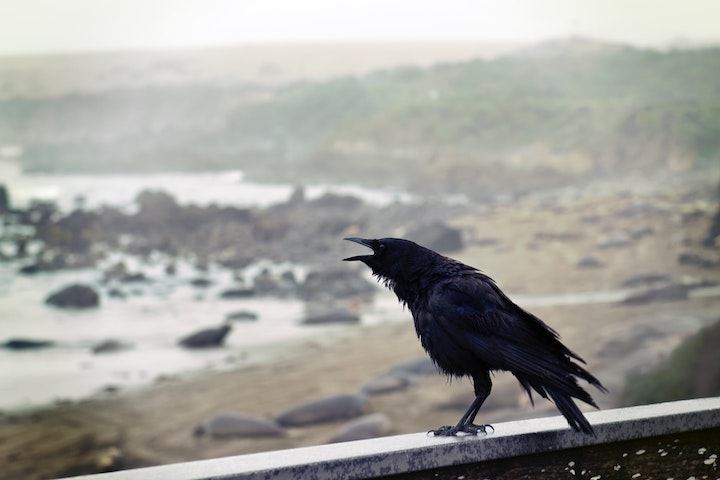
\includegraphics{assets/sample/crow.jpg}

\hypertarget{activity-introductory-readings-video}{%
\subsection*{Activity: Introductory Readings \& Video}\label{activity-introductory-readings-video}}
\addcontentsline{toc}{subsection}{Activity: Introductory Readings \& Video}

\begin{reflect}
\begin{itemize}
\tightlist
\item
  Read \ldots{}\\
\item
  Watch this short informative video that helps you understand the competitive environment by using the case of Amazon books Vs. Independent bookstores.
\end{itemize}

\href{https://www.youtube.com/watch?v=XIt7dEmo4D8}{Watch: \emph{The Competitive Environment Explained}}

Questions to Consider

After watching the above video, consider the following questions:

\begin{itemize}
\tightlist
\item
  \ldots{}\\
\item
  \ldots{}
\end{itemize}

\textbf{Note:} \emph{Learning activities in this course are ungraded, unless specified. They are designed to help you succeed in your assessments in this course, so you are strongly encouraged to complete them.}
\end{reflect}

\hypertarget{topic-2-title}{%
\section{Topic 2 Title}\label{topic-2-title}}

{[}add content{]}

\hypertarget{topic-3-title}{%
\section{Topic 3 Title}\label{topic-3-title}}

{[}add content{]}

\hypertarget{unit-1-summary-1}{%
\section*{Unit 1 Summary}\label{unit-1-summary-1}}
\addcontentsline{toc}{section}{Unit 1 Summary}

{[}add content{]}

\hypertarget{assessment-8}{%
\section*{Assessment}\label{assessment-8}}
\addcontentsline{toc}{section}{Assessment}

\begin{assessment}
{Assessment 1 Title}

\begin{itemize}
\tightlist
\item
  Do a thing\\
\item
  Do another thing
\end{itemize}

{Assessment 2 Title}

\begin{itemize}
\tightlist
\item
  Do a thing\\
\item
  Do another thing
\end{itemize}

\textbf{Note:} \emph{This is an example of a note pertaining to an assessment}
\end{assessment}

\hypertarget{checking-your-learning-4}{%
\subsection*{Checking your Learning}\label{checking-your-learning-4}}
\addcontentsline{toc}{subsection}{Checking your Learning}

\begin{progress}
Now that you have completed the learning activities and assignments for this unit, check the unit learning outcomes below to see if you are able to do the following:

\begin{itemize}
\tightlist
\item
  Describe\ldots{}\\
\item
  Contrast\ldots{}\\
\item
  Analyze\ldots{}\\
\item
  Determine\ldots{}\\
\item
  Create\ldots{}
\end{itemize}

Feel free to review topics more in depth or continue on to the next unit.
\end{progress}

\begin{caution}
\textbf{Sample courses:}

\begin{itemize}
\tightlist
\item
  \href{https://ba-leadership.github.io/ldrs375/}{LDRS 375}\\
\item
  \href{https://ba-leadership.github.io/ldrs440/}{LDRS 440}
\end{itemize}
\end{caution}

\hypertarget{course-credits}{%
\chapter*{Course Credits}\label{course-credits}}
\addcontentsline{toc}{chapter}{Course Credits}

\hypertarget{course-contributors}{%
\section*{Course Contributors}\label{course-contributors}}
\addcontentsline{toc}{section}{Course Contributors}

\hypertarget{curriculum-developer}{%
\subsection*{Curriculum Developer}\label{curriculum-developer}}
\addcontentsline{toc}{subsection}{Curriculum Developer}

\begin{center}\rule{0.5\linewidth}{0.5pt}\end{center}

\hypertarget{course-instructors}{%
\subsection*{Course Instructors}\label{course-instructors}}
\addcontentsline{toc}{subsection}{Course Instructors}

\hypertarget{copyright-credits}{%
\section*{Copyright \& Credits}\label{copyright-credits}}
\addcontentsline{toc}{section}{Copyright \& Credits}

\textbf{Copyright © 2023 Trinity Western University. All rights reserved.}

The content of this course material is the property of Trinity Western University (TWU) and is protected by copyright law worldwide. This material may be used by students enrolled at TWU for personal study purposes only.

TWU seeks to ensure that any course content that is owned by others has been appropriately cleared for use in this course. Anyone wishing to make additional use of such third party material must obtain clearance from the copyright holder.

\hypertarget{course-development-team}{%
\subsection{Course Development Team}\label{course-development-team}}

Course Writer:
Instructional Designer:
Production Team:
Department Chair:
Dean:

Trinity Western University
22500 University Drive
Langley, BC, Canada \textbar{} V2Y 1Y1

\hypertarget{references}{%
\chapter*{References}\label{references}}
\addcontentsline{toc}{chapter}{References}

The following are key references used in this course. \textbf{\emph{Check with your course syllabus for required readings.}}

  \bibliography{book.bib}

\end{document}
